% !TeX root = ../../thesis.tex
\chapter{Introduction}\label{ch:introduction}

% Illustration on how to refer to your papers when using biblatex
% (see second line in thesis.tex to activate biblatex)
%\definecolor{shadecolor}{gray}{0.85}
%\begin{shaded}
%This chapter was previously published as:\\
%\fullcite{VandenBroeck2011IJCAI}
%\newpage
%\end{shaded}

Biodegradable (bioabsorbable) implants provide temporary support for tissues, where the implants completely dissolve and are absorbed by the body during or after tissue healing, avoiding several drawbacks of permanent implants \cite{Gao2022}. The application of biodegradable metallic biomaterials \cite{Zheng2014, Liu2019, Han2019}, including magnesium \cite{Zhao2017,Zhen2013,Willumeit-Roemer2019}, zinc \cite{Venezuela2019,Mostaed2018}, and iron \cite{Schinhammer2010}, has become more prominent for over a decade in various biomedical engineering and tissue engineering disciplines. Among the mentioned materials, magnesium (Mg) is the most studied metal \cite{Esmaily2017}, the reason for which is its suitable mechanical and chemical properties for biomedical applications. Although poor corrosion resistance of Mg is a limiting factor for its application as light structural material, like in the transportation industry, it becomes an interesting characteristic when it comes to the biodegradable materials field for cardiovascular and orthopedic applications \cite{Heublein2003,Staiger2006,Walker2014}. The first clinical usage of Mg was reported in 1878, but a renewed interest in it has grown significantly in the last 15-20 years \cite{Esmaily2017}. From the clinical and biomedical perspective, two major concerns about using Mg in clinics are the release of hydrogen gas and surface alkalization due to Mg dissolution \cite{Cecchinato2015}. These issues are commonly addressed by alloying, biocompatible coating and surface modification \cite{Esmaily2017}. This chapter includes an overview of biodegradable materials with a focus on Mg, the history of their usage in medical applications, a description of the chemistry of Mg biodegradation, and various computational models aiming to capture this chemistry.

\section{Biodegradable metals}

It has been a very long time since metals have started being employed as implant materials to support, reinforce, repair, or replace damaged tissues and organs. Historically speaking, iron dental implants were discovered in the remains of a European who perished at the end of the first century AD or the start of the second century \cite{Crubzy1998}. Moreover, gold has been used for the same application in China since ancient times. With more development in materials science and engineering, inert materials such as titanium alloys, cobalt alloys, and stainless steel are widely used nowadays in biomedical implants and devices. However, there are certain drawbacks to these materials in medical applications:

\begin{itemize}
\item
The release of metallic ions from implants fabricated with these materials can lead to various side effects in the surrounding tissues such as inflammation.
\item
In some cases, such as for temporary fixation in cardiovascular and orthopedics applications, implant presence is unnecessary after the healing process. Moreover, removing the implant via a secondary surgery may not be a practical solution, causing suffering and pain to the patient again.
\item
The difference between the elastic modulus of these materials and the surrounding tissues can lead to various mechanical integrity issues. For instance, in the case of bone, this difference causes stress shielding effect, where the implant acts as a shield preventing the bone from receiving enough mechanical load needed for bone remodeling and growth. Additionally, this may cause further mechanical loosening of the implant and secondary bone fracture.
\end{itemize}

Biodegradable implants would be a great solution to the issues mentioned above. Implants fabricated from biodegradable materials gradually disappear and get absorbed by the body. With more attention to employing these materials in clinical applications, more research studies were conducted to investigate their various aspects. Initially, degradable polymers (such as polylactic acid) were used for this purpose, but later studies showed that they might stimulate the aseptic inflammation of surrounding tissues \cite{Gao2022}. Besides, the mechanical properties of polymer materials are not acceptable in load-bearing applications. As a result, biodegradable metals gained more attention in orthopedics where Mg is the most suitable candidate due to its elastic modulus (41-45 GPa) being closest to that of natural bone (2-30 GPa) \cite{Wang2020a}. In addition to this, especially for bone healing applications, the released metallic ions during the degradation process contribute to the metabolism of the underlying biological process. For example, Mg is one of the most abundant ions found in the bone, and Mg cations have a beneficial impact on the metabolism of enzymes in the bone regeneration process. Similarly, iron (Fe) plays a key role in oxygen transport in the body, and zinc (Zn) positively influences the physiological functions of bone healing and the formation of different transcriptional factors \cite{Wegener2020,Gasior2021,Han2020,Levy2017,Liu2015}.


\section{Magnesium as a biodegradable material}

From the corrosion science perspective, Mg is an active material with a relatively low standard electrode potential of $-2.37\text{V}$, meaning that Mg and its alloys have high corrosion/degradation rate \cite{Gao2022}. This property makes Mg and Mg-based alloys a biodegradable metal in biomedical applications, where the materials undergo corrosion in biological and physiological conditions and disappear during or after the damaged tissue is repaired. 

From the biological perspective, Mg can contribute positively to the human body's metabolism to improve health. A normal adult body contains $20-28\text{g}$ of Mg, from which $27\%$ is distributed in muscles, $65\%$ in bone, and the rest in blood and other tissues \cite{Vormann2003}. Additionally, Mg contributes to more than 300 enzyme reactions in the body \cite{Elin1988}. Extra Mg not needed by the body metabolism is transported via the circulatory system and excreted through the bladder, without causing any major side effect \cite{Wang2020a}.

The first application of Mg for biomedical purposes was recorded in 1878 by Hues, who made artificial radial arteries from Mg and suggested that Mg can be beneficial for the treatment of ovariectomy and hemorrhoids \cite{Gao2022}. Payr performed successful animal experiments using Mg tubular vascular connectors in 1900, after which the vessels were reformed, and vascular thickness returned to its normal range after 16 days of implantation \cite{Witte2010}. This started a wide range of usage of Mg for cardiovascular applications, a recent example of which is the work by Ikeo et al. for designing V-shaped vascular clips made of Mg-Zn-Ca alloy \cite{Ikeo2016}. In this work, the ductility of Mg was reported to be an added advantage for bearing large plastic deformations that these clips experience. In a relevant study, Erbel et al. implanted 71 stents made of Mg alloys in the coronary arteries of 63 patients. The results showed a similar efficiency and safety for Mg stents to that of other metallic stents \cite{Erbel2007}. Moreover, Mg stents degraded without any problem after four months. This type of study resulted in acquiring the CE mark for the next generation of Mg stents in Europe \cite{Sotomi2017,GarciaGarcia2018}.

The history of usage of Mg in orthopedics applications started very similarly to its vascular applications. In the study by Payr mentioned above, he also stated that Mg can improve the bone healing rate \cite{Witte2010}. Six years later, in 1906, the first Mg-based implant was used by Lambotte for fixation of a fracture case \cite{lambotte1909technique,lambotte1932utilisation}. This study was followed by many other studies in the last century, the results of which confirmed that Mg could facilitate the bone healing process. However, these studies also demonstrated that the hydrogen gas released during the biodegradation of Mg could lead to inflammation. Furthermore, since Mg's rate of degradation is high, the tissues may not receive enough support before the implants vanish \cite{Witte2010}. These issues made the Mg-based implants less common compared to inert metals for orthopedics applications. But, in recent decades, these implants gained more attention thanks to enormous research studies on the biodegradation of Mg to control its side effects and degradation behavior. In 2005, the possibility of using Mg for orthopedics implants was proposed by Witte et al. \cite{Witte2005}, a suggestion supported by the results of animal studies on femoral implants manufactured from Mg alloys (AZ31, AZ91, WE43, and LAE442). After this study, a wide variety of research works were conducted to investigate the efficiency of Mg-based implants for orthopedics applications \cite{Wang2020,Huang2020,Zhao2017}. Fig. \ref{fig:intro_applications} shows the current usage of Mg-based implants and medical devices divided into three categories: commercially approved, on clinical trials, and potential applications \cite{Han2019}.

\begin{figure}
\centering
\medskip
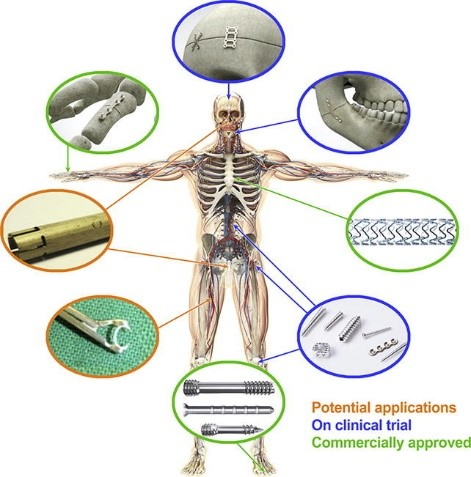
\includegraphics[width=0.6\textwidth]{applications.jpg}
\caption[Various potential applications of Mg as a biodegradable biomaterial]{Various potential applications of Mg as a biodegradable metallic biomaterial for cardiovascular and orthopedic implants and devices \cite{Han2019}.} 
\label{fig:intro_applications}
\end{figure}


\section{Chemistry of biodegradation of magnesium}

\newglossaryentry{PBS}{name={PBS},description={phosphate buffered saline}}
\newglossaryentry{SBF}{name={SBF},description={simulated body fluid}}
\newglossaryentry{HBSS}{name={HBSS},description={Hank's balanced salt solution}}
\newglossaryentry{EBSS}{name={EBSS},description={Earle's balanced salt solution}}
\newglossaryentry{MEM}{name={MEM},description={minimum essential medium}}
\newglossaryentry{DMEM}{name={DMEM},description={Dulbecco's modified Eagle's medium}}

The biodegradation behavior of Mg is investigated in corrosion tests, in which the selection of the corrosive media plays an important role since it affects the underlying chemical reactions \cite{Mei2020}. By considering the main application of the biomaterial, which can be tissue engineering scaffolds, vascular stents, or orthopedic fixation devices, the corrosive media can be selected to be a representative of the service environment. The most basic form of the medium is a saline (NaCl) solution, in which the degradation rate is the highest possible \cite{Mei2020}. More complex solutions can be used to mimic the behavior of the body environment by taking into account more body fluid components, the most popular of which are Ringer's solution, \gls{PBS} (phosphate buffered saline), \gls{SBF}s (simulated body fluids), \gls{HBSS} (Hank's balanced salt solution), and Earle's balanced salt solution (\gls{EBSS}) \cite{Mei2020}. Adding more organic components to the solution will prepare it to simulate cell culture conditions. The common media for this purpose are \gls{MEM} (Minimum Essential medium) and \gls{DMEM} (Dulbecco's modified Eagle's medium) \cite{Mei2020}. Fig. \ref{fig:components} summarizes various commonly used corrosive media for testing biodegradable metals along with their main components  \cite{Mei2020}.


\begin{figure}
\centering
\medskip
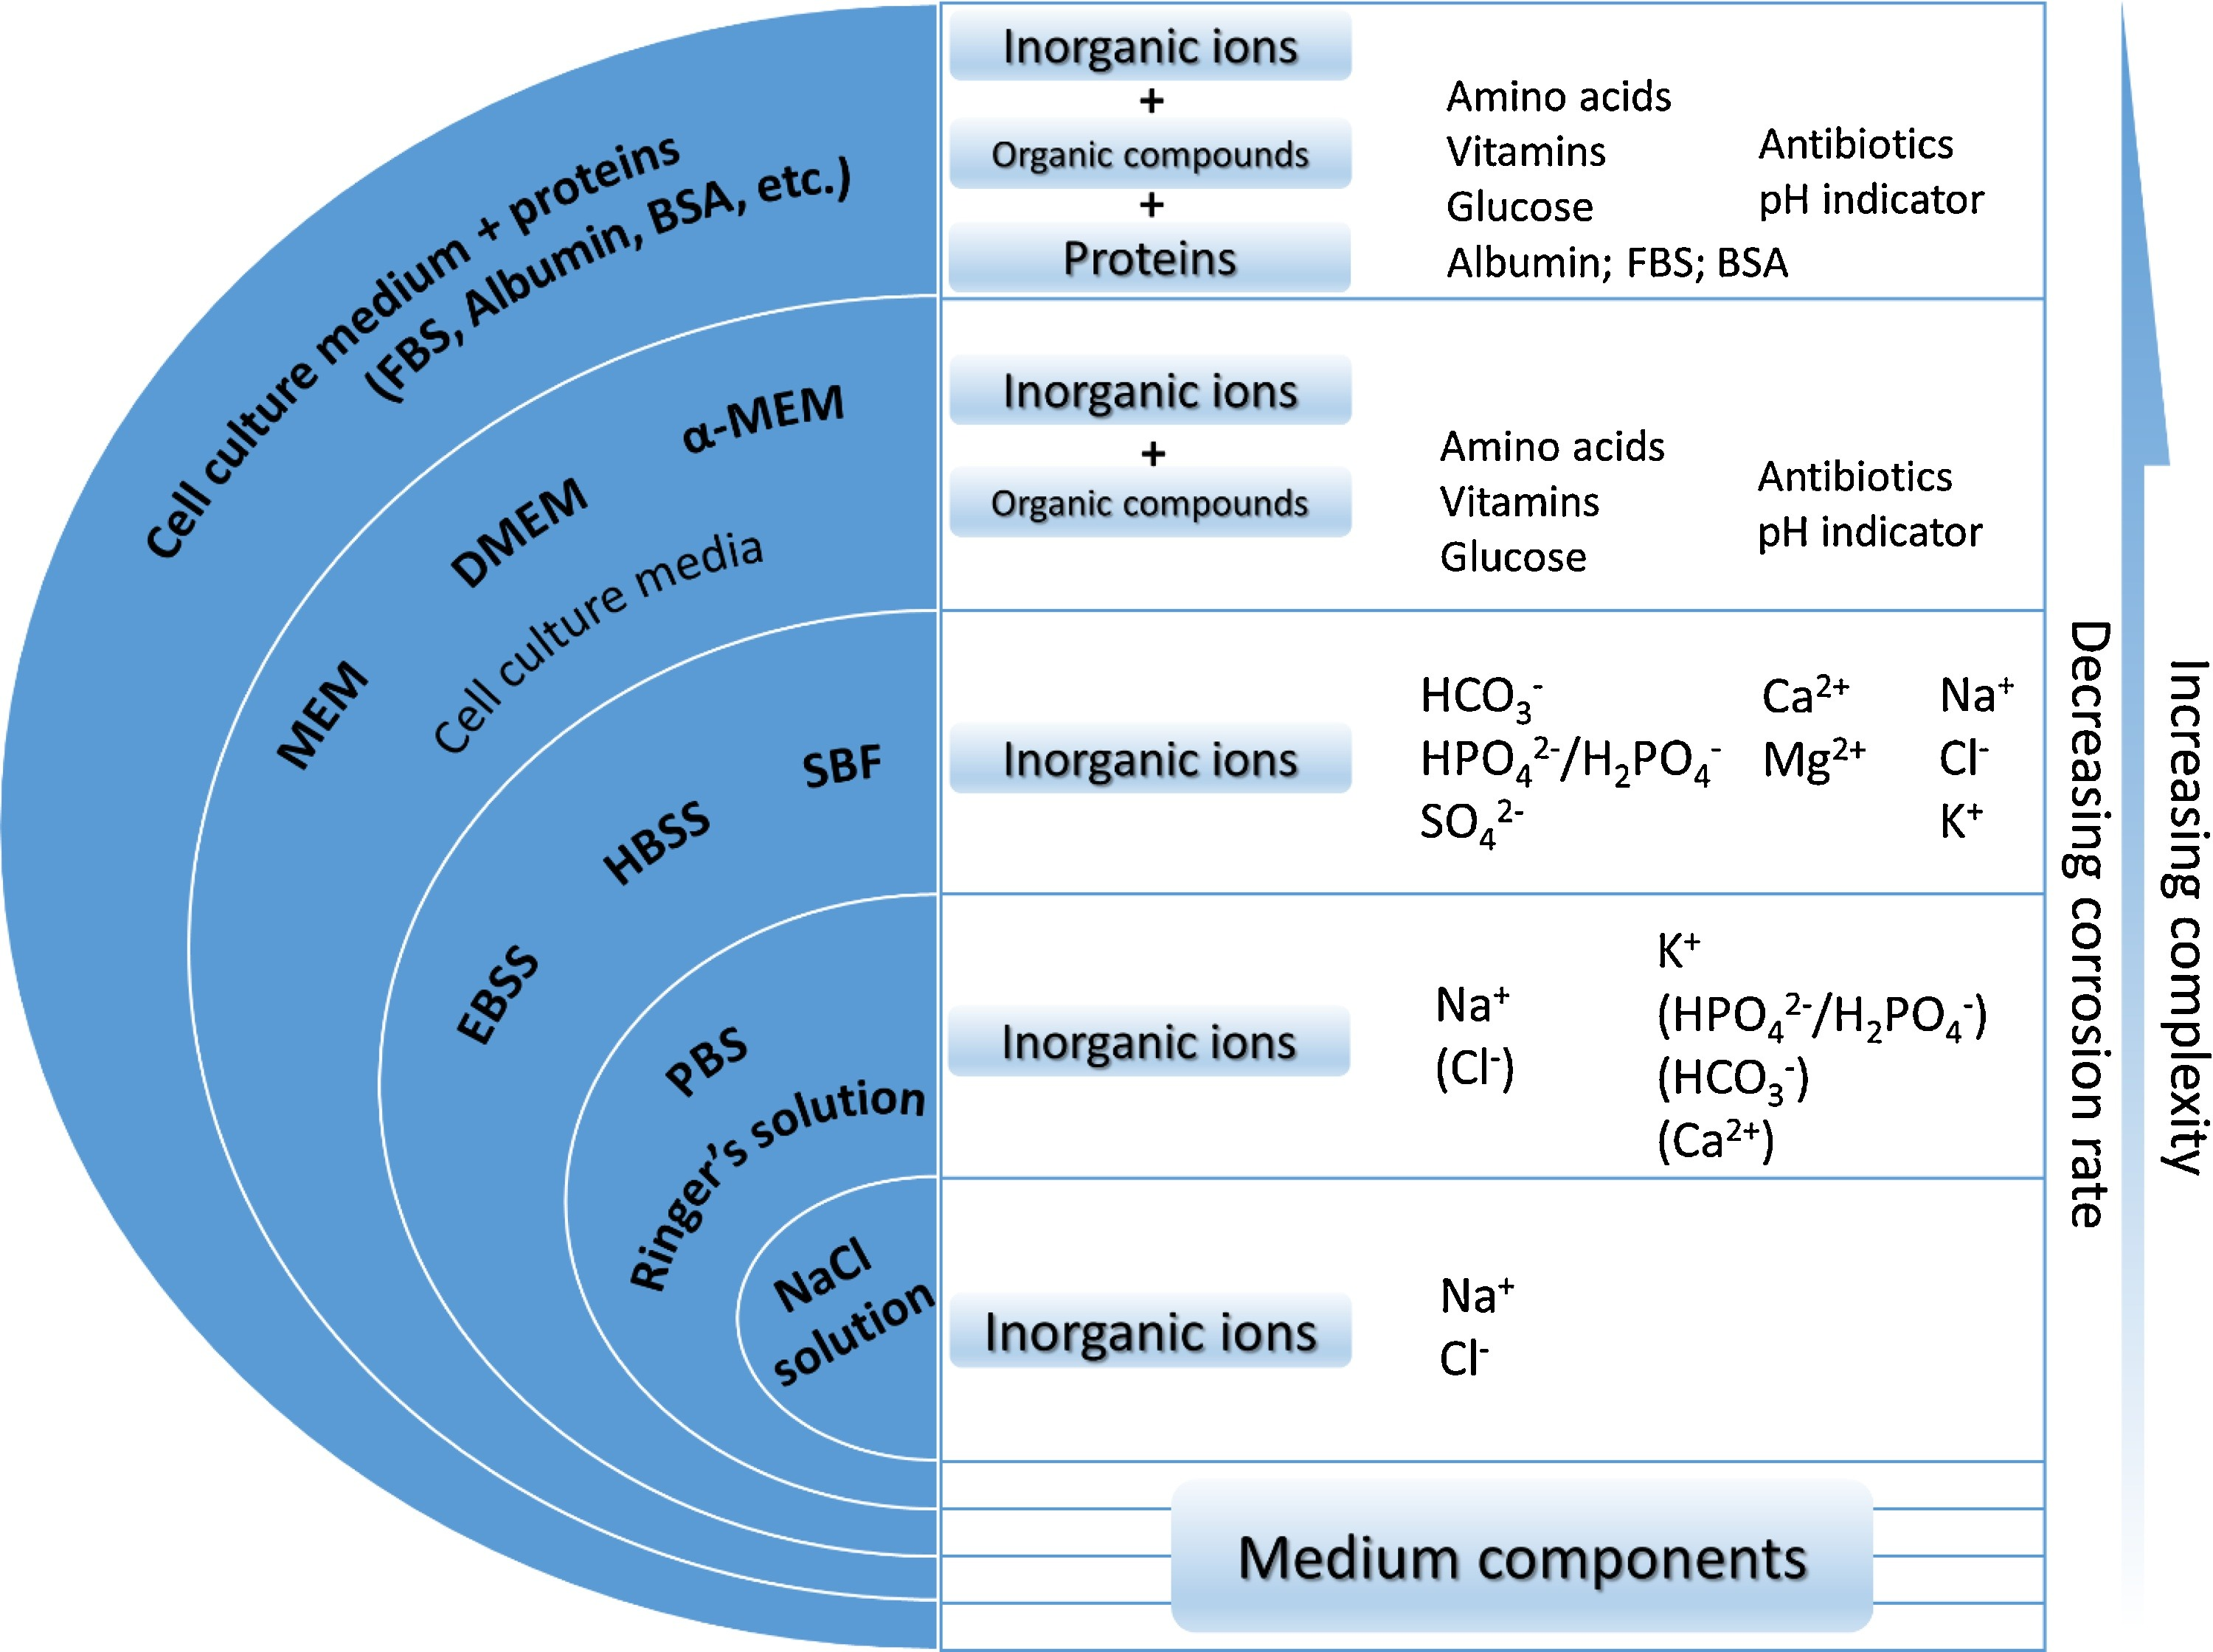
\includegraphics[width=1.0\textwidth]{components.jpg}
\caption[Commonly used corrosive media for testing biodegradable metals]{A schematic representation of commonly used corrosive media for testing biodegradable metals, sorted by their complexity from the chemical perspective from bottom to top \cite{Mei2020}.} 
\label{fig:components}
\end{figure}

Various studies have already investigated the effect of different components in the aforementioned corrosive media on the degradation behavior of Mg materials \cite{Mei2019,Zeng2014,Johnston2017, Lamaka2018,Mei2019a}. In addition to the presented chemical components, it has been shown that synthetic pH buffers (such as Tris and HEPES) contribute to the biodegradation rate of Mg \cite{Mei2019}. The investigations on the effect of different inorganic components, including carbonate, phosphate, sulfate and calcium, show these components' effective contribution to the degradation rate. However, the corrosion protection resulting from the mutual effect of carbonate, phosphate and calcium has been emphasized more \cite{Mei2019,Lamaka2018}.




The most common solution for performing corrosion tests on Mg is saline (NaCl) solution, in which the material undergoes aggressive corrosion due to higher electrochemical activities \cite{Hadzima2014,Lu2019}. In a typical aqueous solution, the major corrosion reactions occurring can be written as detailed below \cite{Li2020,Atrens2015}.

\newglossaryentry{HER}{name={MD},description={hydrogen evolution reaction}}
\newglossaryentry{ORR}{name={ORR},description={oxygen reduction reaction}}

Main, hydrogen evolution reaction (\gls{HER}):
\begin{equation}
\mathrm{Mg}+2 \mathrm{H}_{2} \mathrm{O} \rightarrow \mathrm{Mg}(\mathrm{OH})_{2}+\mathrm{H}_{2}.
\end{equation}

Secondary, oxygen reduction reaction (\gls{ORR}):
\begin{equation}
2 \mathrm{Mg}+2 \mathrm{H}_{2} \mathrm{O}+\mathrm{O}_{2} \rightarrow 2 \mathrm{Mg}(\mathrm{OH})_{2}.
\end{equation}

In this situation, the corrosion products forming on the corroded surface of Mg consist mainly of $\mathrm{Mg}(\mathrm{OH})_{2}$ and $\mathrm{MgO}$, and the pH in regions close to this surface remains alkaline. In the presence of chloride ions in the saline medium, the formed corrosion product may be broken or bypassed, leading to an increased degradation rate.
\begin{equation} \label{eq:break_react_intro}
\mathrm{Mg}(\mathrm{OH})_{2}+2 \mathrm{Cl}^{-} \rightarrow \mathrm{Mg}^{2+}+2 \mathrm{Cl}^{-}+2 \mathrm{OH}^{-}
\end{equation}
\begin{equation} \label{eq:break_react_mgo_intro}
\mathrm{MgO}+ \mathrm{Cl}^{-} + \mathrm{H}_{2} \mathrm{O} \rightarrow \mathrm{Mg}^{2+}+ \mathrm{Cl}^{-}+ 2\mathrm{OH}^{-}
\end{equation}


The main advantage of using a saline solution for corrosion tests compared to more complex media is that the absence of inorganic ions like carbonate, phosphate, sulfate and calcium allows for investigating the corrosion behavior without concerning possible effect caused by the interaction of these chemical components. On the other hand, the main weakness of saline solution is that it cannot represent the complexity of real body fluid, and as a result, a more complex medium is required to investigate such conditions. To address this issue, more complex saline solutions, such as PBS, are widely used for assessing the applicability of Mg alloys in more complex conditions from the chemical perspective \cite{Schille2011,Xue2012}. Despite the mentioned limitations, corrosion tests in saline solution are still contributing to understanding intrinsic degradation properties of Mg. 


The term "simulated body fluid" is generally used to refer to solutions containing inorganic ions of human serum and interstitial fluid \cite{Mei2020}. The commonly used corrosive media in this regard are \gls{SBF}, \gls{HBSS}, and \gls{EBSS}, which all include the same inorganic components yet with a slight difference in their concentrations. A typical composition of these media is chloride, carbonate, phosphates, sulfate and calcium. The individual effect of these components on the rate of degradation of Mg has been extensively studied, where it has been observed that carbonate and phosphate slow down the rate whereas the effect of sulfate is negligible \cite{Johnston2017,Mei2019a}. The concentration of $\mathrm{HCO}_{3}^{-}$ affects the pH buffering capacity and the degradation rate of Mg simultaneously \cite{Xin2011}. The effect of calcium ions is more complex because it does not contribute to Mg corrosion directly. Fig. \ref{fig:reactions_intro} briefly summarizes the various reactions and formed precipitation compositions of the mentioned media for testing the degradation behavior of Mg \cite{Mei2020}.


\begin{figure}
\centering
\medskip
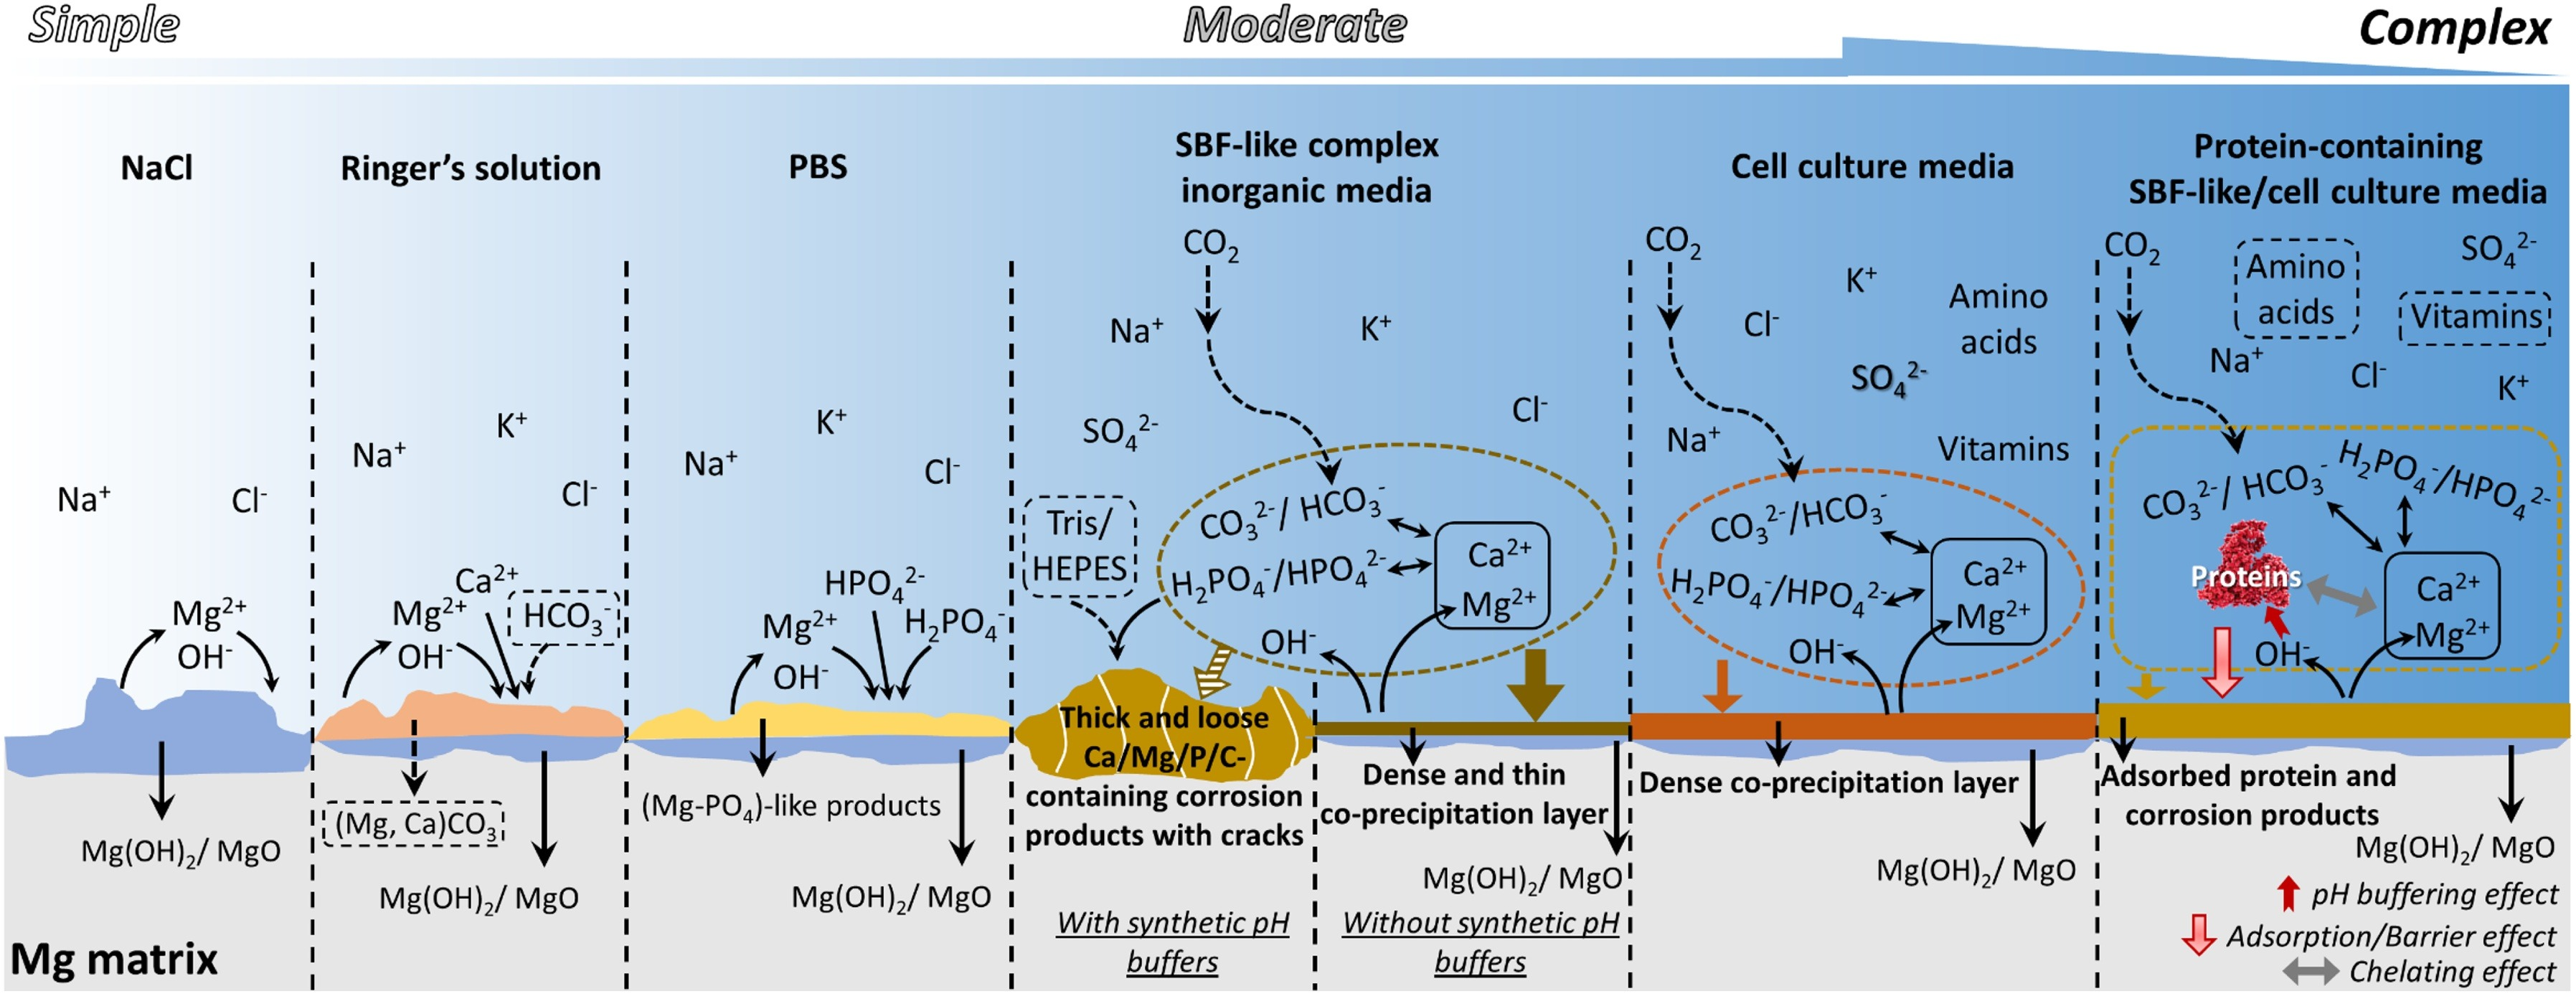
\includegraphics[width=1.0\textwidth]{reactions.jpg}
\caption[Mg biodegradation behavior in commonly used test solutions]{A schematic representation of Mg biodegradation behavior in commonly used solutions for corrosion tests of biodegradable metals \cite{Mei2020}.} \label{fig:reactions_intro}
\end{figure}


There are various evaluation techniques for measuring the degradation rate of Mg, among which the weight loss, hydrogen evolution, potentiodynamic polarization, and electrochemical impedance spectroscopy are the commonly used ones. Generally speaking, the method used for evaluating the degradation rate can affect the reported behavior. For example, it has been shown that in \gls{HBSS}, the measured corrosion rate of Mg is lower (slower) when evaluated using hydrogen evolution in comparison to the rate found by direct weight loss measurements \cite{Johnston2015,Johnston2019}, which can be due to the secondary dissolution of evolved hydrogen. Moreover, oxygen consumption due to secondary \gls{ORR} can affect the volume of evolved gas, which is more significant for media with slower degradation rates such as \gls{HBSS} and \gls{MEM} \cite{Wang2020}. Table \ref{tab:methods_intro} summarizes the advantages and shortcomings of widely used techniques for measuring degradation rate \cite{Mei2020}. 


\begin{table}[h]
\caption[Summary of various common methods to assess the degradation rate of Mg]{Summary of various common methods to assess the degradation rate of Mg \cite{Mei2020}}
\medskip
\resizebox{\textwidth}{!}{%
\begin{tabular}{p{0.3\textwidth}p{0.5\textwidth}p{0.5\textwidth}}
\hline
Test method &
  Advantages &
  Shortcomings \\ \hline
Weight loss &
  \begin{tabular}[p{0.4\textwidth}]{@{}p{0.45\textwidth}}High reliability\\ Direct measurement\\ Easily controlled test environment\end{tabular} &
  \begin{tabular}[p{0.4\textwidth}]{@{}p{0.45\textwidth}}Non-continuous. Does not reveal varying corrosion rate throughout the immersion\\ Low sensitivity at the initial stages\end{tabular} \\ \hline
Hydrogen evolution &
  \begin{tabular}[p{0.4\textwidth}]{@{}p{0.45\textwidth}}Continuous\\ Can be automated\\ Can be performed in closed eudiometers\end{tabular} &
  \begin{tabular}[p{0.4\textwidth}]{@{}p{0.45\textwidth}}Performed in open environment in most cases\\ Might show underestimated values of corrosion rate due to secondary \gls{ORR} and solubility of $\mathrm{H}_2$ in aqueous media\end{tabular} \\ \hline
Potentiodynamic polarization &
  Fast measurement &
  \begin{tabular}[p{0.4\textwidth}]{@{}p{0.45\textwidth}}Non-continuous\\ Open environment measurement in most cases\\ Very often low correlation with long-term weight loss measurements\end{tabular} \\ \hline
Electrochemical impedance spectroscopy &
  \begin{tabular}[p{0.4\textwidth}]{@{}p{0.45\textwidth}}Continuous\\ In situ investigation of protective properties of forming corrosion products\end{tabular} &
  Performed in open environments in most cases
\\  \hline
\end{tabular}}
\label{tab:methods_intro}
\end{table}


\section[Computational modeling of biodegradation]{Computational modeling of biodegradation\footnote{This section is partially based on a manuscript prepared to be submitted:\\S. Mukherjee, S. Mandal, M. Barzegari, F. Perez-Boerema, B. Liang, E. Sadeghian Dekhord, L. Groeneveldt, L. Geris, ``In silico design and optimization of mesoscopic and macroscopic properties of additively manufactured scaffolds: applications in skeletal tissue engineering.''}}


Besides experimental approaches to investigate the properties of biodegradable metallic implants and scaffolds, computational modeling of the biodegradation process and behavior can be used as an efficient tool to design the next generation of medical devices and implants \cite{Boland2015}. In addition to traditional modeling approaches for mechanics of materials, it is possible to take advantage of well-developed principles of modeling transport phenomena and numerical simulations to investigate the biodegradation process computationally \cite{SanzHerrera2019}.

\newglossaryentry{WSS}{name={WSS},description={wall shear stress}}
\newglossaryentry{CD}{name={CD},description={continuous damage}}

Computational models of the biodegradation process vary from a basic implementation of the process to comprehensive mathematical models that capture multiple aspects of the degradation phenomenon. In the category of simplified corrosion models, Gao et al. performed a quantitative study on the change of mechanics during the biodegradation of Mg alloys for cardiovascular applications \cite{Gao2018}. Liu et al. developed a fluid dynamics model to characterize the effect of the induced wall shear stress (\gls{WSS}) on the biodegradation mechanism of Mg stents \cite{Liu2018}. They investigated the effect of blood flow velocity and dynamic environment on the degradation of cardiovascular stents. Boland et al. studied the mechanical performance of Mg stents for the treatment of coronary artery diseases using a computational model \cite{Boland2019}. Gartzke et al. proposed a degradation model for the corrosion of Mg alloys coupled with mechanical analysis, allowing them to study the change of mechanical properties during the biodegradation process \cite{Gartzke2020}. Another common category of studies in this regard is continuous damage (\gls{CD}) simulations, in which geometrical discontinuities get translated into the reduction of materials. Despite the limitation of this technique for modeling biodegradation, such as more focus on the mechanical integrity rather than on the fundamental phenomena, it has been used for various relevant studies, such as Gastaldi et al. \cite{Gastaldi2011} and Shi et al. \cite{Shi2021}. 

Among the relevant studies, mass transfer-related models were more successful in representing the biodegradation process mathematically. Indeed, the approach of constructing models based on the well-formulated transport phenomena equations and then solving the derived equations using appropriate numerical schemes has been followed in recent years to study biodegradation. Ahmed et al. derived a set of mathematical equations to capture the chemical reactions occurring in Mg degradation \cite{Ahmed2017}, in which the detailed mathematical equations provided a proper insight into the effect of different chemical components on the biodegradation of Mg \textit{in vitro}. Grogan et al. developed a model to correlate the mass flux of the metallic ions in the biodegradation interface to the velocity of the interface, used to simulate the degradation of complex geometries of Mg-based stents \cite{Grogan2014}. Similarly, Shen et al. developed a theoretical model to predict the degradation behavior of Mg alloys in orthopedic implants \cite{Shen2019}. Their 3D model had a high agreement with \textit{in vitro} corrosion test results.

\newglossaryentry{LSM}{name={LSM},description={level-set method}}

One of the important applications of biodegradation models is to investigate the change of shape and morphology of the implants and medical devices over time. To this end, appropriate interface capturing methods should be used to track the corrosion interface during the biodegradation process. Bajger et al. developed a mathematical model to study the degradation of Mg implants by reaction-diffusion equations and level-set method (\gls{LSM}), which enabled them to track the geometrical changes of the implant during degradation \cite{Bajger2016}. Similarly, Sanz-Herrera et al. developed a comprehensive computational model as a tool for Mg implant design \cite{Sanz-Herrera2018}. They combined multiple diffusion-reaction equations to study the change of concentration of the chemical components that play an essential role in \textit{in vitro} biodegradation of Mg implants. A summary of the studies mentioned above is represented in Table \ref{tab:intro_review}. The reader is encouraged to refer to \cite{Albaraghtheh2022} for a more complete list of recent published mechanistic and phenomenological models of the biodegradation process of Mg-based implants.

\clearpage

\newglossaryentry{FVM}{name={FVM},description={finite volume method}}
\newglossaryentry{FEM}{name={FEM},description={finite element method}}
\newglossaryentry{UMAT}{name={UMAT},description={user-defined material model}}
\newglossaryentry{FSI}{name={FSI},description={fluid-structure interaction}}
\newglossaryentry{ALE}{name={ALE},description={arbitrary Lagrangian-Eulerian}}
\newglossaryentry{USDFLD}{name={USDFLD},description={user-defined field}}
\newglossaryentry{CFD}{name={CFD},description={computational fluid dynamics}}
\newglossaryentry{MOL}{name={MOL},description={method of lines}}

\begin{table}[h]
\caption[Summary of the recently-developed computational models of the degradation process]{Summary of the recently-developed computational models of the degradation process of Mg-based biomaterials and some of their key characteristics. FEM: Finite Element Method; CFD: Computational Fluid Dynamics; FVM: Finite Volume Method; MOL: Method of Lines; FSI: Fluid-Structure Interaction; ALE: Arbitrary Lagrangian-Eulerian.}
\medskip
\resizebox{1\textwidth}{!}{
%\begin{tabular}{lllllll}
\begin{tabular}{p{0.18\textwidth}p{0.15\textwidth}p{0.15\textwidth}p{0.17\textwidth}p{0.15\textwidth}p{0.15\textwidth}p{0.05\textwidth}}
\hline
\textbf{Biological system} &
  \textbf{Modeled device} &
  \textbf{Material} &
  \textbf{Basis of degradation}  &
  \textbf{Software used} &
  \textbf{Modeling   method} &
  \textbf{Ref} \\ \hline
Artery &
  Vascular stent &
  Mg Alloy AZ31B &
  Surface corrosion &
  ABAQUS &
  \gls{FEM}, \gls{UMAT} &
  \cite{Gao2018} \\ \hline
Artery &
  Vascular stent &
  Mg Alloy WE43 &
  Surface corrosion &
  ANSYS Fluent &
  \gls{CFD}, \gls{FSI}, \gls{FVM} &
  \cite{Liu2018} \\ \hline
Remodeling artery &
  Vascular stent &
  Mg Alloy AZ31 &
  Uniform and pitting   corrosion &
  ABAQUS &
  \gls{FEM}, \gls{USDFLD} &
  \cite{Boland2019} \\ \hline
Artery &
  Coronary stents &
  Mg alloys AZ31,   AZ61, AZ80, ZK60 and ZM21 &
  Surface and stress   corrosion &
  ABAQUS &
  \gls{CD}, \gls{FEM} &
  \cite{Gastaldi2011} \\ \hline
Bone &
  Orthopedic implants &
  Pure Mg &
  Surface corrosion by   considering biphasic layers &
  MATLAB &
  Mass transfer, \gls{MOL} &
  \cite{Ahmed2017} \\ \hline
Artery &
  Vascular stent &
  Mg Alloy AZ31 &
  Surface corrosion &
  ABAQUS &
  Diffusion model,   \gls{ALE}, \gls{FEM} &
  \cite{Grogan2014} \\ \hline
Bone &
  Orthopedic pins &
  Mg alloys Mg-1Ca and   Mg-3Ge &
  Surface corrosion &
  ABAQUS &
  Diffusion model,   \gls{FEM}&
  \cite{Shen2019} \\ \hline
Hip bone &
  Orthopedic implant &
  Pure Mg &
  Surface corrosion &
  In-house, FreeFEM &
  Reaction-diffusion   model, \gls{LSM}, \gls{FEM} &
  \cite{Bajger2016} \\ \hline
Bone &
  Orthopedic screws &
  Mg alloy &
  Surface corrosion &
  In-house &
  Reaction-diffusion   model, \gls{FEM} &
  \cite{Sanz-Herrera2018} \\ \hline
Bone &
  Porous scaffolds &
  Mg Alloy LAE442 &
  Surface corrosion &
  ABAQUS &
  \gls{FEM}, {UMAT} &
  \cite{Gartzke2020} \\ \hline
Artery &
  Vascular stent &
  Mg Alloy AZ31 &
  Surface corrosion &
  ABAQUS &
  \gls{CD}, \gls{FEM}, \gls{UMAT} &
  \cite{Shi2021}
\end{tabular}}
\label{tab:intro_review}
\end{table}

\clearpage

The approach taken by Bajger et al. was followed in the current thesis, in which an improved model was developed by considering more chemical components and phenomena, allowing us to perform a more accurate validation using \textit{in vitro} data. Although the biodegradation models are getting more mature and more promising for simulating experimental situations, their integration into other models, such as mechanical stability analysis or neotissue growth, to construct fully-coupled models has remained a challenge. Solving this challenge will enable future models to replicate complex \textit{in vivo} conditions more accurately \textit{in silico}.


%% Some dummy code to get at least 1 entry in the nomenclature.
%\nomenclature{$\Theta$}{A nice symbol}
%Introducing some symbol: $\Theta$.
%
%% Some dummy code to get at least 1 entry in the list of
%% abbreviations.
%\newglossaryentry{md}{name={MD},description={molecular dynamics}}
%Introducing an acronym: \gls{md}.




%%%%%%%%%%%%%%%%%%%%%%%%%%%%%%%%%%%%%%%%%%%%%%%%%%
% Keep the following \cleardoublepage at the end of this file, 
% otherwise \includeonly includes empty pages.
\cleardoublepage

% vim: tw=70 nocindent expandtab foldmethod=marker foldmarker={{{}{,}{}}}

